\documentclass{beamer}
%\usepackage[usenames,dvipsnames]{xcolor}

\usepackage{_defsAndPackages675notation}
\usepackage{_defsAndPackages675beamer}

\begin{document}

\title{\alg{Linear Methods for Regression}}
\subtitle{\classTitle}
%\author{\alg{Darren Homrighausen, PhD}}
%\institute{\classTitle}
\date{}



\begin{frame}
\maketitle
%\titlepage
%\begin{figure}[h!]
%  \centering
%  \includegraphics[width=1in]{.../figures/CSU_logo2.eps}
%\end{figure}
%
\organization
%
\end{frame}

\begin{frame}
\frametitle{The Setup}
Suppose we have data 
\[
\data = \{ (X_1 , Y_1), (X_2 , Y_2), \ldots, (X_n , Y_n) \},
\]
where 
\begin{itemize}
	\item $X_i \in \mathbb{R}^p$  are the \alg{features} 

	{\scriptsize (or \alg{explanatory variables} or \alg{predictors} or \alg{covariates}.  NOT INDEPENDENT VARIABLES!)}
\item $Y_i \in \mathbb{R}$ are the \alg{response} variables.

	{\scriptsize (NOT DEPENDENT VARIABLE!)}
\end{itemize}
\vsp

Our goal for this class is to find a way to explain (at least approximately) the \alo{relationship}
between $X$ and $Y$.
\vsp
\end{frame}

\begin{frame}
\frametitle{Prediction risk for regression}
Given the \alo{training data} $\data$, we want to predict some independent \alo{test data} $Z = (X,Y)$

\vsp
This means forming a $\hat f$, which is a function of both the range of $X$ and the training data $\data$, 
which provides predictions $\hat Y = \hat f(X)$.

\vsp
The quality of this prediction is measured via the prediction risk\footnote{ Note: sometimes we integrate with
respect to $\data$ only, $Z$ only, neither (loss), or both.}
\[
R(\hat{f}) = \P_{\data,Z}(Y - \hat{f}(X))^2.
\]

We know that the \alo{regression function}, $f_*(X) = \P[Y | X]$, is the best possible predictor.  


\vsp
However, it is {\it unknown}.
\end{frame}
%
%\begin{frame}
%\frametitle{Prediction risk for regression}
%Note that $R(\hat{f})$ can be written as
%\[
%R(\hat{f}) = \int \textrm{bias}^2(x) d\P_X + \int \textrm{var}(x) d\P_X + \sigma^2
%\]
%where
%\begin{align*}
%\textrm{bias}(x) & = \P\hat{f}(x) - f_*(x)\\
%\textrm{var}(x) & = \V\hat{f}(x) \\
%\sigma^2 & = \P(Y - f_*(X))^2
%\end{align*}
%\end{frame}


\begin{frame}
\frametitle{Prediction risk for regression}



\begin{columns}[T]
    \begin{column}{.7\textwidth}
Note that $R(\hat{f})$ can be written as
\[
R(\hat{f}) = \int \textrm{bias}^2(x) d\P_X + \int \textrm{var}(x) d\P_X + \sigma^2
\]
where
\begin{align*}
\textrm{bias}(x) & = \P\hat{f}(x) - f_*(x)\\
\textrm{var}(x) & = \V\hat{f}(x) \\
\sigma^2 & = \P(Y - f_*(X))^2
\end{align*}

\vsp
\script{As an aside, this decomposition applies to much more general loss functions\footnote{
\Cite{Variance and Bias for General Loss Functions}{James}{Machine Learning 2003}}}
\blfootnote{(http://home.ubalt.edu/ntsbarsh/Business-stat/)}
\end{column}
    \begin{column}{.3\textwidth}
\includegraphics[width=.6in,trim= 10 50 180 5,clip]{../figures/biasVariance} \\
\includegraphics[width=.6in,trim= 180 40 10 5,clip]{../figures/biasVariance}

\end{column}
\end{columns}
\end{frame}


\begin{frame}
\frametitle{Bias-variance tradeoff}
This can be heuristically thought of as
\[
\textrm{Prediction risk} = \textrm{Bias}^2 + \textrm{Variance}.
\]

There is a natural conservation between these quantities

\vsp
Low bias $\rightarrow$ complex model $\rightarrow$ many parameters $\rightarrow$ high variance

\vsp
The opposite also holds

\script{Think: $\hat f \equiv 0$.}

\vsp
We'd like to `balance' these quantities to get the best possible predictions
\end{frame}

\begin{frame}
\frametitle{Bias-variance tradeoff}
 \begin{figure}
 \centering
 \includegraphics[width=3in,trim=0 50 0 20,clip]{../figures/regression_biasVar.pdf}   \\
  \caption*{Model Complexity $\nearrow$}
  \end{figure}
\end{frame}


\begin{frame}
\frametitle{Training error and risk estimation}
Using $\hat{\P}$, and writing $\ell_f(Z) = (f(X) - Y)^2$, we can form the \alg{training error}
\[
\hat{R}(f) = \hat{\P}\ell_f = \frac{1}{n}\sum_{i=1}^n \ell_f(Z_i) = \frac{1}{n}\sum_{i=1}^n (f(X_i) - Y_i)^2.
\]
\vsp

In many cases in applied statistical applications, this \alg{plug-in} estimator is used

\script{Think of how many techniques rely on an unconstrained minimization of squared error, or 
maximum likelihood, or estimating equations, or ...}

\vsp
This sometimes has disastrous results
\end{frame}


\begin{frame}[fragile]
\frametitle{Example}
Let's suppose $\data$ is drawn from

\begin{verbatim}
n = 30
X = (0:n)/n*2*pi
Y = sin(X) + rnorm(n,0,.25)
\end{verbatim}
\vsp

Now, let's fit some polynomials to this data.  

\vsp
We consider the following models:
\begin{itemize}
\item[-] Model 1:  $f(X_i) = \beta_0 + \beta_1 X_{i}$
\item[-]Model 2: $f(X_i) = \beta_0 + \beta_1 X_{i} + \beta_2 X_{i}^2 + \beta_3 X_{i}^3$
\item[-]Model 3: $f(X_i) = \sum_{k=0}^{10} \beta_k X_{i}^k$
\item[-]Model 4: $f(X_i) = \sum_{k=0}^{n-1} \beta_k X_{i}^k$
\end{itemize}
Let's look at what happens...
\end{frame}

\begin{frame}
\frametitle{Example}
\begin{columns}[T]
    \begin{column}{.55\textwidth}
  \includegraphics[width=2.5in,trim=0 15 0 20,clip]{../figures/polynomialExample.pdf}
  \end{column}
    \begin{column}{.45\textwidth}
 The $\hat{R}$'s are: 
 \begin{itemize}
 \item[] \textcolor{black}{$\hat{R}$(Model 1) = 10.98}
 \item[] \textcolor{red}{$\hat{R}$(Model~2)~=~2.86}
 \item[] \textcolor{blue}{$\hat{R}$(Model 3)~=~2.28}
 \item[] \textcolor{green}{$\hat{R}$(Model 4) = 0}
 \end{itemize}
\vsp

What about predicting new observations (\textcolor{magenta}{$\Delta$})?
    \end{column}
  \end{columns}
  \end{frame}


\begin{frame}
\frametitle{Example}
\begin{columns}[T]
    \begin{column}{.55\textwidth}
  \includegraphics[width=2.5in,trim=0 15 0 20,clip]{../figures/polynomialExample.pdf}
  \end{column}
    \begin{column}{.45\textwidth}
 \begin{itemize}
 \item \textcolor{black}{Black model} has low variance, high bias
 \item \textcolor{green}{Green model} has low bias, but high variance
 \item \textcolor{red}{Red model} and \textcolor{blue}{Blue model} have intermediate
 bias and variance.
 \end{itemize}
\vsp

We want to balance these two quantities.
    \end{column}
  \end{columns}
\end{frame}

\begin{frame}
\frametitle{Bias vs. Variance}
\begin{columns}[T]
    \begin{column}{.5\textwidth}
  \includegraphics[width=2.3in,trim=0 15 0 20,clip]{../figures/polynomialExample.pdf}
  \end{column}
    \begin{column}{.5\textwidth}
    \begin{tabular}{c}
  \includegraphics[width=2.3in,trim=0 15 0 20,clip]{../figures/regression_biasVarColoredLines.pdf}   \\
  {\footnotesize Model Complexity $\nearrow$}
  \end{tabular}
   \end{column}
  \end{columns}
\vsp

\end{frame}

\transitionSlide{A linear model}

\begin{frame}
\frametitle{A linear model}
Specify 
%\footnote{We'll revisit this later with Projection Pursuit/Neural Nets.} 
functions $\phi_k:\R^p \rightarrow \R$, $k=1,\ldots,K$

\[
\X = 
\left[
\phi_k(X_i)
\right]
=
\left[
\begin{array}{c}
\Phi(X_{1})^{\top} \\
\Phi(X_{2})^{\top} \\
\vdots    \\
\Phi(X_{n})^{\top} \\
\end{array}
\right]
 \in R^{n\times K},
\]
where $\Phi(\cdot)^{\top} = (\phi_1(\cdot), \ldots, \phi_K(\cdot))$.
%Commonly, $x_{i1} = 1$, which encodes an intercept term in the model.
\vsp

Here,  $f_*(X) = f_{*,\Phi_K}(X)  + f_{*,\Phi_K^c}(X)$ and
\[
\Phi_K = \{ f : \exists (\beta_k)_{k=1}^K \textrm{ such that } f = \sum_{k=1}^K \beta_k \phi_k = \beta^{\top} \Phi\}
\]
and 
\[
f_{*,\Phi_K} = \argmin_{f \in \Phi_K} \P\ell_f.
\]

\vsp
The function $f_{*,\Phi_K}$ is known as the \alg{linear oracle}
\end{frame}

%\begin{frame}
%\frametitle{A linear model: Example 1}
%Suppose $f_* \in \F$, where $\F$ is a Hilbert space with norm induced by the inner product $\langle \cdot, \cdot \rangle$. 
%\vsp
%
%Let $(\phi_k)_{k=1}^\infty$ be an orthonormal basis for $\F$
%
%\vsp
%Write 
%\[
% f_* = \sum_{k=1}^\infty \langle f_*, \phi_k \rangle \phi_k =  \sum_{k=1}^\infty \beta_k \phi_k
%\]
%
%Then, if we state that $f_* \in \beta(m,c)$
%\end{frame}

\begin{frame}
\frametitle{A linear model: Ordinary Least Squares}
Let $K = p$ and define $\phi_k$ to be the coordinate projection map
\vsp

 That is, for $x = (x_1,\ldots,x_p)^{\top}$
 \[
 \phi_k(x) \equiv x_k
 \]
 \vsp
 
 Then we recover the usual linear regression formulation
\[
\X = 
\left[
\begin{array}{cccc}
X_{11} & X_{12} & \cdots & X_{1p} \\
X_{21} & X_{22} & \cdots & X_{2p} \\
\vdots & & \\
X_{n1} & X_{n2} & \cdots & X_{np} \\
\end{array}
\right]
=
\left[
\begin{array}{cccc}
X_{1}^{\top} \\
X_{2}^{\top} \\
\vdots    \\
X_{n}^{\top} \\
\end{array}
\right].
\]
Commonly, $X_{i1} = 1$, which encodes an intercept term in the model.
\end{frame}

\begin{frame}
\frametitle{A linear model: Orthogonal basis expansion}
Suppose $f_* \in \F$, where $\F$ is a Hilbert space with norm induced by the inner product $\langle \cdot, \cdot \rangle$. 
\vsp

Let $(\phi_k)_{k=1}^\infty$ be an orthonormal basis for $\F$

\vsp
Write 
\[
 f_* = \sum_{k=1}^\infty \langle f_*, \phi_k \rangle \phi_k =  \sum_{k=1}^\infty \beta_k \phi_k
\]

\vsp
Then we can estimate $f_{*,\Phi_K}$ by finding the coefficients of the projection on $\Phi_K$.  
\vsp

By Parseval's theorem\Note for Hilbert spaces\note, this induces an \alo{approximation} error of $\sum_{k=K+1}^{\infty} \beta_k^2$.

\vsp
This is small if $f_*$ is smooth 

\script{for instance, if $f_*$ has $m$ derivatives, 
then $\beta_k \asymp k^{-m}$}
\end{frame}

\begin{frame}
\frametitle{A linear model: Neural Nets}
Let 
\[
\phi_k(x)  = \sigma(\alpha_k^{\top}x + b_k),
\]
where $\sigma(x) = 1/(1 + e^{-x})$ is the \alg{sigmoid} function.
\vsp

Then $f_{*,\Phi_K}$ is called an\footnote{More on this later}:
\[
\textrm{``single-layer feed-forward neural network model with linear output''} 
\]
\end{frame}

\begin{frame}
\frametitle{A linear model: Radial basis functions}
Let 
\[
\phi_k(x)  = e^{-||\mu_k - x||_2^2/\lambda_k}.
\]

Then $f_{*,\Phi_K}$ is called an\footnote{More on this later}:
\[
\textrm{``Gaussian radial-basis function estimator'}.
\]

This turns out to be a parametric form of a more general technique known as \alg{Gaussian process regression}.
\end{frame}

\begin{frame}
\frametitle{The limits of linearity}
Each of these methods have parameters to choose:
\begin{itemize}
\item Ordinary least squares: how large is $p$?
\item Orthogonal basis expansion: which basis and how large is $K$?
\item Neural Nets: The activation function $\sigma$, the directions $\alpha_k$,  bias terms $b_k$, as well as $K$.
\item Radial basis functions: The choice of the kernel (here we have used Gaussian), the centroids $\mu_k$, 
the scales $\lambda_k$, and $K$ again.
\end{itemize}

\vsp
We would like the data to inform these parameters

\vsp
However, this requirement turns the problem from a straightforward 
optimization problem (with closed form solution) into a combinatorially hard \alo{nonlinear problem} (In fact, NP hard)

\vsp
 In practice, we use greedy algorithms, iterative schemes, and convex relaxation to solve the
 \alo{computational} problem. 
 
 \vsp
  The \alo{statistical} problem is still fundamentally projection
 onto a function space, with the function space estimated from the data.
\end{frame}

\begin{frame}
\frametitle{Low-dimensional linear regression ($K \leq n$)}
Supposing that the functions $\phi_k$ are {\it known}, 
we can form the \alg{least-squares estimator} by
``plugging in'' the empirical measure for the unknown true measure
\[
\hat{f}= \argmin_{f \in \Phi_K} \hat{\P}\ell_f,
\]
where, for each  $f \in \Phi_K$, there is a coefficient vector $\beta$ such that 
$\ell_f(Z) = (X^{\top}\beta - Y)^2$.
\vsp

In this case, 
\[
\hat{f}(X) = X^{\top} \hat \beta,
\]
where 
\[
\hat\beta = \X^{\dagger}Y = (\X^{\top} \X)^{-1} \X^{\top} Y
\]
and $\X^{\dagger}$ is the Moore-Penrose pseudo inverse\note.

\vsp
In particular, the fitted values are $\X\hat\beta = H Y$, where $H$ is the orthogonal projection onto the 
column space of $\X$
\end{frame}

\begin{frame}
\frametitle{Low-dimensional linear regression ($K \leq n$)}
We can examine the first and second moment properties of $\hat\beta$

Focusing on the $f_{*,\Phi_K} = \beta^{\top}\Phi$ component\footnote{This is important! In claiming $\hat\beta$ is 
`unbiased' we are asserting either that: (1)  $f_{*,\Phi_K^c} \equiv 0$ or (2) it is unbiased for the coefficients of
the linear oracle $f_{*,\Phi_K}$.} 
\begin{align}
\label{eq:bias}
\E \hat\beta  & =  \beta \qquad (\textrm{unbiased})\\
\label{eq:var}
\V \hat\beta  & =  \X^{\dagger} (\V Y) (\X^{\dagger})^{\top}  = \V[Y_i] (\X^{\top}\X)^{-1} 
\end{align}

The Gauss-Markov theorem assures us that this is the best linear \alo{unbiased} estimator of $\beta$

\script{That is, equation (\ref{eq:var}) is minimized subject to equation (\ref{eq:bias})}

\vsp
Also, it is the maximum likelihood estimator under a homoskedastic, independent Gaussian model

\script{Hence, it is asymptotically efficient}
\vsp

Does that necessarily mean it is any good?
\end{frame}

\begin{frame}
\frametitle{Low-dimensional linear regression ($K \leq n$)}
Write $\X = U D V^{\top}$ for the SVD of $\X$
\vsp

Then $\V \hat\beta \propto (\X^{\top}\X)^{-1}  = V D^{-2} V^{\top}$.
\vsp

We know that the diagonal elements of $D$, $d_j$, are then lengths of the axes of the ellipse induced by $\X$
\vsp

Also, suppose we are interested in estimating $\beta$,
\[
\E|| \hat\beta - \beta||_2^2  =  \textrm{trace}(\V\hat\beta) \propto \sum_{j=1}^p \frac{1}{d_j^2}
\]
\vsp

Even in the low-dimensional case, we can do arbitrarily badly if $d_p \approx 0$.
\end{frame}


\begin{frame}
\frametitle{Returning to polynomial example: Bias}
Using a Taylor's series, for all $x$
\[
\sin(x) = \sum_{q = 0}^\infty \frac{(-1)^qx^{2q+1}}{(2q + 1)!} 
\]
Therefore, higher order polynomial models will reduce the approximation (bias) part
\end{frame}

\begin{frame}
\frametitle{Returning to polynomial example: Variance}
However, the least squares solution is given by solving $Ax = b$, where
\[
A =
\begin{bmatrix}
1 & X_1 & \ldots & X_1^{K-1} \\
   & \vdots && \\
 1 & X_n & \ldots & X_n^{K-1} \\
\end{bmatrix},
\]
is the associated Vandermonde\Note matrix. 

\vsp
This matrix is well known for being numerically unstable as $K$ increases 
\script{Letting $A = UDV^{\top}$, this means that $d_1/d_K \rightarrow \infty$} 

\vsp 
Hence\footnote{This should be compared with the variance computation in equation (\ref{eq:var})}
\[
||(A^{\top}A)^{-1}||_2 = \frac{1}{d_K^2}
\]
grows larger, where here $||\cdot||_2$ is the \alg{spectral (operator) norm}\Note
\end{frame}

\begin{frame}
\frametitle{Returning to the polynomial example}
\begin{figure}
\centering
  \includegraphics[width=2.5in,trim=0 15 0 20,clip]{../figures/polynomialExample.pdf}
\end{figure}
\end{frame}


\begin{frame}
\frametitle{Many questions left to answer}
\begin{itemize}
\item Is a linear estimator appropriate (what is the size of $f_{*,\Phi_K^c}(X)$)?
\item What is a good choice of $\phi_k$?
\item How well does $\argmin_{f \in \Phi_K} \hat{\P}\ell_f$ mimic $\argmin_{f \in \Phi_K} \P\ell_f$?
\item What is a good choice of $K$?  Are all the $\phi_k$ needed?
\item What happens if we want to choose $K > n$?
\end{itemize}

\end{frame}

\transitionSlide{Subset selection, regularization, and risk estimation}

\begin{frame}
\frametitle{Subset selection and regularization}
For now, let's assume we are doing ordinary least squares, and hence the design (feature) matrix is $\X \in \R^{n \times p}$.

\vsp
We want to do model selection for at least two reasons:
\begin{itemize}
\item \smallCapGreen{Prediction accuracy:} Can essentially {\it always} be improved by introducing some bias 
\item \smallCapGreen{Interpretation:} A large number of features can sometimes be distilled into a smaller number that comprise the  ``big (little?) picture''
\end{itemize}

We will address three related ideas 
\begin{itemize}
\item \smallCapGreen{Model selection:} Selection of only some of the original $p$ features
\item \smallCapGreen{Dimension reduction/expansion:} Creation of new features to help with prediction
\item \smallCapGreen{Regularization:} Add constraints to optimization problems to provide stabilization
\end{itemize}
\end{frame}


\begin{frame}
\frametitle{Risk estimation}
Reminder:  Prediction risk is
\[
R(f) = \P_{Z,\data} \ell_f \leftrightarrow \textrm{Bias} + \textrm{Variance}
\]
The overridding theme is that we would like to add a judicious amount of bias to get \alo{lower} risk

\vsp
As $R$ isn't known, we need to estimate it

\vsp
As discussed, $\train = \hat\P\ell_f$ isn't very good

\script{In fact, one tends to not add bias when estimating $R$ with $\hat\P\ell_f$}
\end{frame}

\begin{frame}
\frametitle{Risk estimation: a general form}
Assume that we get a new draw of the training data, $\data^0$, such that $\data \sim \data^0$ and
\[
\data = \{(X_1,Y_1), \ldots, (X_n,Y_n)\} \quad \textrm{and} \quad \data^0 = \{(X_1,Y_1^0), \ldots, (X_n,Y_n^0)\}
\]

\vsp
If we make a small compromise to risk, we can form a sensible suite of risk estimators

\vsp
To wit, letting $Y^0 = (Y_1^0,\ldots,Y_n^0)^{\top}$, define 

\[
R_{in} = \E_{Y^0 | \data}  \hat\P_{\data^0}  \ell_{\hat{f}}= \frac{1}{n} \sum_{i=1}^n \E_{Y^0 | \data} \ell(\hat{f}(X_i),Y_i^0)
\]
\vsp

Then the \alg{average optimism} is
\[
\opt = \E_Y [ R_{in} - \train]
\]
Typically, $\opt$ is positive as $\train$ will underestimate the risk
\end{frame}

\begin{frame}
\frametitle{Risk estimation: a general form}
It turns out for a variety of $\ell$ (such as squared error and 0-1)
\[
\opt = \frac{2}{n} \sum_{i=1}^n \textrm{Cov}(\hat f(X_i),Y_i)
\]
\vsp

Therefore, we get the following expression of risk
\[
 \E_Y R_{in} = \E_Y \train + \frac{2}{n} \sum_{i=1}^n \textrm{Cov}(\hat f(X_i),Y_i),
\]
which has unbiased estimator (i.e. $\E_Y \gic =  \E_Y R_{in}$)
\[
\gic = \train + \frac{2}{n} \sum_{i=1}^n \textrm{Cov}(\hat f(X_i),Y_i)
\]
\end{frame}

\begin{frame}
\frametitle{Degrees of freedom}
We call the term (where $\sigma^2 = \V Y_i$)
\[
\df = \frac{1}{\sigma^2} \sum_{i=1}^n \textrm{Cov}(\hat f(X_i),Y_i)
\]
the \alg{degrees of freedom}

\script{This is really the \alo{effective number of parameters}, with some caveats}

\vsp
Our task now is to either estimate or compute $\opt$ to produce $\opthat$ and form:
\[
\gichat = \train + \opthat
\]

\vsp
This leads to AIC, BIC, Cp, and others

\script{See the homework for an exploration of this topic}
\end{frame}

\transitionSlide{ Comparing probability measures  }

\begin{frame}
\frametitle{ Kullback-Leibler}

We've produced a suite 
of (generalized) information criteria

\vsp
Suppose we have data $Y$ that comes from the probability density function $f$.

\vsp
What happens if we use the probability density function $g$ instead?

\vsp
One central idea is \alg{Kullback-Leibler}\Note discrepancy\footnote{This has many features of a distance, but is not a true distance as $KL(f,g) \neq KL(g,f)$.} \begin{align*}
KL(f,g) & = \int \log\left( \frac{f(y)}{g(y)} \right)f(y) dy \\
& \propto
-\int \log (g(y)) f(y) dy \qquad \textrm{(ignore term without $g$)}\\
& = 
-\P_f [\log (g(Y))] 
\end{align*}

This gives us a sense of the \alo{loss} incurred by using $g$ instead of $f$. 
\end{frame}

\begin{frame}
\frametitle{ Kullback-Leibler discrepancy  }
Usually, $g$ will depend on some parameters, call them $\theta$
\vsp

\emphasis{8.75cm}{Example:}{In regression, we can specify $f = N(X^{\top} \beta, \sigma^2)$ for a fixed 
(true)\footnotemark  $\beta$, and let $g_\theta = N(X^{\top}\beta,\sigma^2)$ over all $\theta \in \R^p\times\R^+$}

\vsp
As $KL(f,g_\theta) = -\P_f [\log (g(Y;\theta))]$, we minimize this over $\theta$.

\vsp
Again, $f$ is unknown, so we minimize $-\log (g(Y;\theta))$ instead.  This is the maximum likelihood value
\[
\hat{\theta}_{ML} = \argmax_\theta g(y;\theta)
\]

\footnotetext{We actually don't need to assume things about a true model nor have it be nested in
the alternative models.}
\end{frame}

\begin{frame}
\frametitle{ Kullback-Leibler discrepancy  }
Now, to get an operational characterization of the KL divergence at the ML solution
\[
-\P [\log (g(Y;\hat\theta_{ML}))]
\]
we need an approximation (don't know $f$, still)

\vsp
This approximation\footnote{See ``Multimodel Inference'' Burnham, Anderson (2004)} is exactly AIC\Note:
\[
\textrm{AIC} = -2\log (g(Y;\hat\theta_{ML})) + 2|\hat\beta_{ML}|
\]

\emphasis{8.75cm}{Example:}{
Let $\log(g(y;\theta)) = -\frac{n}{2}\log(2\pi\sigma^2) - 
\frac{1}{2\sigma^2}||Y - \X\beta||_2^2$ 

\smallCapGreen{$\sigma^2$ known:}
$\hat\beta = \X^{\dagger}Y$
\[
\textrm{AIC} \propto n \train/\sigma^2 + 2p.
\]
\smallCapGreen{$\sigma^2$ unknown:}
$\hat\beta = \X^{\dagger}Y$, $n\hat\sigma^2 = (I - \X\X^{\dagger})Y = n\train$}
\[
\textrm{AIC} \propto n \log(\train) + 2p 
\]


\end{frame}

\transitionSlide{Cross-validation}

\begin{frame}
\frametitle{A different approach to risk estimation}
 Let $(X_0,Y_0)$ be a test
observation, identically distributed as an element in $\data$, but also \alo{independent} of $\data$.
\vvsp

\emphasis{7cm}{Prediction risk:}{$R(f) = \E (Y_0 - f(X_0))^2$}
\vsp

Of course, the quantity $(Y_0 - f(X_0))^2$ is an unbiased estimator of $R(f)$ and hence we could
estimate $R(f)$
\vsp

However, \alo{we don't have any such new observation}

\vsp
Or do we?

\end{frame}

\begin{frame}
\frametitle{An intuitive idea}
Let's set aside one observation and predict it

\vsp
\emphasis{9cm}{For example:}{Set aside $(X_1,Y_1)$ and fit $\hat{f}^{(1)}$ on $(X_2,Y_2),\ldots,(X_n,Y_n)$. }

{\scriptsize (The notation $\hat{f}^{(1)}$
just symbolizes leaving out the first observation before fitting $\hat{f}$)}
\[
R_1(\hat{f}^{(1)}) = (Y_1 - \hat{f}^{(1)}(X_1))^2
\]

As the left off data point is \alo{independent} of the data points used for estimation, 
\[
\E_{(X_1,Y_1)|\data_{(1)}}R_1(\hat{f}^{(1)})  \stackrel{D}{=} R(\hat f(\data_{n-1}) ) \approx R(\hat f(\data))
\]


\end{frame}

\begin{frame}
\frametitle{Leave-one-out cross-validation}
Cycling over all observations and taking the average produces \alg{leave-one-out cross-validation}

\[
\CV{n}(\hat{f}) =  \frac{1}{n} \sum_{i=1}^n R_i(\hat{f}^{(i)}) = \frac{1}{n} \sum_{i=1}^n (Y_i -  \hat{f}^{(i)}(X_i))^2.
\]

\end{frame}

\begin{frame}
\frametitle{More general cross-validation schemes}
Let $\mathcal{N} = \{1,\ldots,n\}$ be the index set for $\data$
\vsp

Define a distribution $\VV$ over $\mathcal{N}$ with (random) variable $v$
\vsp
 
Then, we can form a general \alg{cross-validation} estimator as
\[
\CVV(\hat f) =  \E_\VV \hat \P_v \ell_{\hat{f}^{(v)}}
\]
\end{frame}

\begin{frame}
\frametitle{More general cross-validation schemes: Examples}
\[
\CVV(\hat f) =  \E_\VV \hat \P_v \ell_{\hat{f}^{(v)}}
\]

\begin{itemize}
\item \smallCapGreen{K-fold:} Fix $V = \{ v_1,\ldots,v_K\}$ such that $v_j \cap v_k = \emptyset$ and 
$\bigcup_j v_j = \mathcal{N}$
\[
\CV{K}(\hat f) = \textcolor{redmain}{\frac{1}{K} \sum_{v \in V}} \textcolor{bluemain}{\frac{1}{|v|} \sum_{i \in v}} \textcolor{greenmain}{(Y_i - \hat{f}^{(v)}(X_i))^2}
\]
\item \smallCapGreen{Bootstrap:} Let $\VV$ be given by the bootstrap distribution over $\mathcal{N}$
\script{that is, sampling with replacement many times}
\item \smallCapGreen{Factorial:} Let $\VV$ be given by all subsets (or a subset of all subsets) of $\mathcal{N}$
\script{that is, putting mass $1/(2^n-2)$ on each subset}
\end{itemize}

\end{frame}

\begin{frame}
\frametitle{More general cross-validation schemes: A comparison}
\begin{itemize}
\item $\CV{K}$ gets more computationally demanding as $K \rightarrow n$
\item The bias of $\CV{K}$ goes down, but the variance increases as $K \rightarrow n$
\item The factorial version isn't commonly used except when doing a `real' data example for a methods
paper
\item  There are many other flavors of CV.  One of them, called ``consistent cross validation'' 
[\smallCapGreen{Homework}] is a recent addition that is designed to work with \alo{sparsifying} algorithms
\end{itemize}
\end{frame}


\transitionSlide{Summary time}

\begin{frame}[fragile]
\frametitle{Risk estimation methods}

\begin{table}
\begin{tabular}{lp{9.5cm}}
   \smallCapGreen{CV}  &  Prediction risk consistent (Dudoit, van der Laan (2005)).  Generally selects a model
   larger than necessary (unproven) \\
   \smallCapGreen{AIC}  & Minimax optimal risk estimator (Yang, Barron (1998)).  Model selection inconsistent$^*$ \\   
   \smallCapGreen{BIC}  &  Model selection consistent (Shao (1997) [low dimensional]. Wang, Li, Leng (2009) [high dimensional]).  
   Slow rate for risk estimation$^*$\\   
\end{tabular}
\end{table}

\script{Stone (1977) shows that $\CV{n}$ and AIC are asymptotically equivalent.}

\script{$^*$Yang (2005) gives an impossibility 
theorem: for a linear regression problem it is impossible for a model selection criterion to be
both consistent and achieve minimax optimal risk estimation}
\end{frame}

\begin{frame}[fragile]
\frametitle{Summary}
The overall scheme is a three(four?)-fold process
\begin{enumerate}
\item Select a method suited to your task
\item Choose a risk estimation method that has the properties that you desire (see next slide)
\item \textcolor<2>{redmain}{Perform the necessary computations to minimize \textcolor{bluemain}{2.} constrained
to be in the family of procedures in \textcolor{bluemain}{1.}}
\item Show theoretically that your procedure has desirable properties
\end{enumerate}
\end{frame}



\transitionSlide{Brief optimization and convexity detour}

\begin{frame}[fragile]
\frametitle{Optimization}
An optimization problem (program) can be generally formulated as
\begin{align}
\textrm{minimize } & F(x) \\
\label{eq:constraint1}
\textrm{subject to } 
& f_j(x) \leq 0 \textrm{ for }  j = 1, \ldots, m \\
\label{eq:constraint2}
& h_k(x) = 0 \textrm{ for }  k = 1, \ldots, q
\end{align}
Here
\begin{itemize}
\item[] $x = (x_1, \ldots, x_n)^{\top}$ are the \alg{parameters}
\item[] $F:\R^n \rightarrow \R$ is the \alg{objective function}
\item[] $f_j,h_k:\R^n \rightarrow \R$ are \alg{constraint functions}
\end{itemize}

\vsp
The \alg{optimal solution} $x^*$ is such that $F(x^*) \leq F(x)$ for any $x^*,x$ that satisfies equations (\ref{eq:constraint1}) and (\ref{eq:constraint2}).
\end{frame}

\begin{frame}[fragile]
\frametitle{Convexity}
The main dichotomy of optimization programs is  \alg{convex} vs. \alg{nonconvex}
\vsp

Generally speaking, a \alg{convex} program is one in which the objective and contraint functions are all convex,
that is $\forall t \in [0,1], \forall x \in D = \left(\bigcap_{j =1}^m \textrm{dom } f_i \right) 
\cap \left(\bigcap_{k=1}^q \textrm{dom } h_k\right) \cap \left(\textrm{dom F}\right)$, and 
$\forall f \in \{ f_1,\ldots, f_m, h_1,\ldots,h_q, F\}$
\[
f(tx + (1-t)x') \leq tf(x) + (1-t)f(x')
\]
This can be thought of (for smooth enough $f$)
\[
f(x') \geq f(x) + (\nabla f|_x)^{\top} (x' - x) 
\]

\emphasis{8cm}{Intuition:}{This means that the function values at a point $x'$ are \alo{above}
the supporting hyperplane given by the tangent space at \alo{any} point $x$}

\end{frame}

\begin{frame}[fragile]
\frametitle{Convexity}
Methods  for convex optimization programs are (roughly) always \alo{global} and \alo{fast}

\vsp
For general nonconvex problems, we have to give up one of these:
\begin{itemize}
\item Local optimization methods that are fast, but need not find global solution
\item Global optimization methods that find global solutions, but
are not always fast (indeed, are often slow)
\end{itemize}
\end{frame}

\transitionSlide{Model selection}
\begin{frame}
\begin{center}
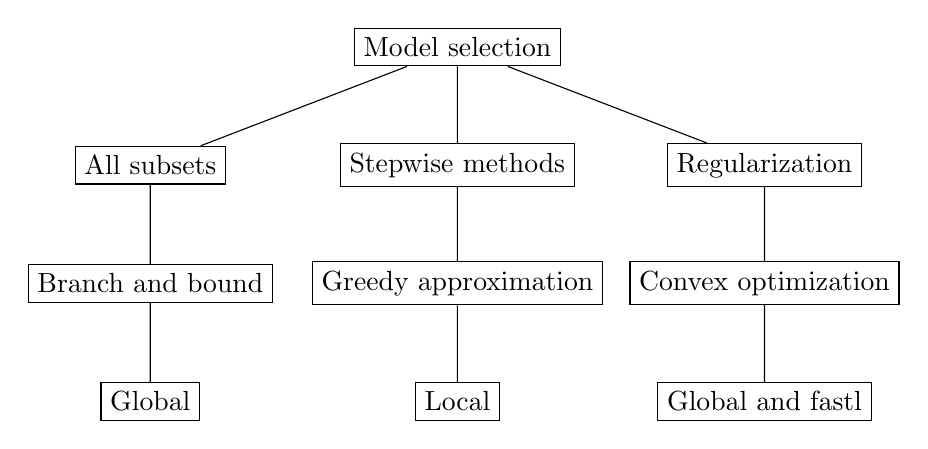
\begin{tikzpicture}
    \tikzstyle{every node}=[rectangle,draw]
    \tikzstyle{level 1}=[sibling distance=39mm] 
    \tikzstyle{level 2}=[sibling distance=23mm]     
    \node {\smallCapGreen{Model selection}}
            child { node {\alr{All subsets}}
            	child { node {\alr{Branch and bound}}
			child { node {\alo{Global}}}
		} 
            }
            child { node {\alr{Stepwise methods}} 
            	child { node {\alr{Greedy approximation}}
			child { node {\alo{Local}}}
		} 
            }
        	   child { node {\alb{Regularization}}           
            	child { node {\alb{Convex optimization}}
			child { node {\alb{Global and fastl}}}
		} 
            }
         ;
\end{tikzpicture}
\end{center}
\vsp

Some comments:
\begin{itemize}
\item[] \alr{Non convex programs}
\item[] \alb{Can be seen as a convex relaxation of the nonconvex program giving all subsets}\footnote{We'll
return to this shortly}
\end{itemize}
\end{frame}


\begin{frame}[fragile]
\frametitle{All Subsets Regression: A Big Problem  (Literally)}
If there are $p$  predictors  then there are \alo{$2^p -1$ possible models} 

\script{Without considering interactions or transformations}

\vsp
In general, this is a nonconvex problem 
\vsp

If $p = 40$
(which is considered a small problem these days), then the number of possible models is
\[
2^{40} -1 \approx 1,099,512,000,000 \Rightarrow \textrm{More than 1 trillion!}
\]

\vsp
If $p = 265$, then the number of possible models is more than the \alo{number of atoms
in the universe}\footnote{It is estimated there are $10^{80}$ atoms in the universe.}

\vsp
We must sift through the models in a computationally feasible way
\end{frame}

\begin{frame}[fragile]
\frametitle{All Subsets Regression}
This can efficiently be computed via the \alr{leaps} package in \alr{R}, using either the 
\alr{leaps} or \alr{regsubsets} functions.

\vsp
This is a specific case of \alg{branch and bound}

\script{The statistical implementation is based on the paper Furnival and Wilson (1974)}
\vsp

It is by far the most widely used tool for solving large scale NP-hard combinatorial optimization problems.

\vsp
Note, however, that though it can speed up the optimization immensely, it cannot reduce the complexity
of the problem (still exponential)


\end{frame}

\begin{frame}[fragile]
\frametitle{Branch and bound}
Let $M = \{M_1,\ldots,M_K\}$ be the set of all possible solutions and a partition comprised of \alg{branches}, respectively.  

\script{Statistically, we think of $M$ as the set of all possible models.}


\vsp

Let $F$ be the objective function and $m_* = \max_{m \in M} F(m)$.

\vsp
For each $M_k$, define
\[
m_k = \max_{m \in M_k} F(m) 
\]
and let $\underline{m}_k, \overline{m}_k $ be a \alo{bracket} such that
\[
 \underline{m}_k \leq m_k \leq \overline{m}_k 
\]
\script{Note that $m_k$ is in general not explicitly constructed}
\vsp

Then
\[
\max_k \underline{m}_k = \underline{m} \leq m_* \leq \overline{m} = \max_k \overline{m}_k
\]
\end{frame}

\begin{frame}[fragile]
\frametitle{Branch and bound}
The main realization is that the \alg{branch} $M_k$ does not need to be explored if
either of the following occur
\begin{itemize}
\item[i.] \smallCapGreen{Bound}
\[
\overline{m}_k \leq \underline{m}
\]
\item[ii.] \smallCapGreen{Optimality}
\[
\max_{m \in M_k} F(m) \textrm{ has been found}
\]
\end{itemize}

The two main questions remain:
\begin{enumerate}
\item How to choose the partition(s)?
\item How to form the upper/lower bounds?
\end{enumerate}


These are very case specific.  Let's return to model selection
\end{frame}

\begin{frame}[fragile]
\frametitle{Branch and bound for model selection}
Let's suppose we set\footnote{Note: we are trying to minimize $F$, not maximize}
\[
F(m) = n \log(\train(\hat\beta_m)) + 2|m| 
\]

For the $M_k$, let
\begin{itemize}
\item[] $m_{k,inf}$ be the largest model contained\footnote{This does not have to be in $M_k$}
 in every model in $M_k$
\item[] $m_{k,sup}$ be a smallest model that contains every model in $M_k$
\end{itemize}

\end{frame}

\begin{frame}[fragile]
\frametitle{Branch and bound for model selection}
\textbf{Example:} Let $x_1, \ldots, x_5$ be covariates

\[
M  = \cup_{k=1}^3 M_k,
\]
where
\begin{align*}
M_1 
& = \{\{x_1,x_3\}, \{x_2\} \}, \\
M_2 
& = \{\{x_2,x_3,x_4\}, \{x_3,x_4\} \}, \\
 M_3 
& = \{\{x_3,x_5\}, \{x_3\} \}, 
\end{align*}
\pause

\begin{itemize}
\item[] $m_{2,inf} = \{x_3,x_4\}$
\item[] $m_{2,sup} = \{x_2,x_3,x_4\}$
\end{itemize}


\end{frame}

\begin{frame}[fragile]
\frametitle{Branch and bound for model selection}
\alo{Reminder:}

For the $M_k$, let
\begin{itemize}
\item[] $m_{k,inf}$ be the largest model contained
 in every model in $M_k$
\item[] $m_{k,sup}$ be a smallest model that contains every model in $M_k$
\end{itemize}
\vsp

Then, $\forall m \in M_k$
\begin{itemize}
\item[] $F(m) \geq n \log(\train(\hat\beta_{m_{k,\sup}})) + 2|m_{k,\inf}| = L_k$  
\item[] $F(m) \leq n \log(\train(\hat\beta_{m_{k,\inf}})) + 2|m_{k,\sup}|  = U_k$ 
\end{itemize}

\end{frame}

\begin{frame}[fragile]
\frametitle{Branch and bound for model selection: An algorithm}
\begin{enumerate}
\item Define a global variable $b = F(m)$ for any $m \in M$

\script{As an aside, every time $F(m)$ is computed, update $b$ if $F(m) < b$} 
\item Partition $M = \{M_1,\ldots,M_K\}$\Note
\item For each $k$, if $L_k > b$, eliminate the branch $M_k$
\item Else, recurse and return to \textcolor{bluemain}{2.}, substituting $M_k$ for $M$
\end{enumerate}

\end{frame}

\begin{frame}[fragile]
\frametitle{(Forward) stepwise selection}
In the likely event that $|M|$ is too large to be searched over exhaustively, a common \alg{greedy}
approximation is the following

\begin{enumerate}
\item Find $b = F(\emptyset)$, where $\emptyset$ is the empty set
\item Search over all $p$ singleton sets and record $m_{1,\min} = \argmin F(m)$.  If $F(m_{1,\min}) < b$ set  $b \leftarrow F(m_{1,\min})$, else return $\emptyset$
\item Now search over all $p-1$ models that contain $m_{1,\min}$ and form $m_{2,\min} = \argmin F(m_{1,\min} \cup \{x_j\})$.
If $F(m_{2,\min}) < b$ set  $b \leftarrow F(m_{2,\min})$, else return $m_{1,\min}$
\item $\cdots$
\end{enumerate}

\end{frame}

\begin{frame}
\frametitle{General stepwise selection}
This algorithm can can adapted to..
\begin{itemize}
\item start with the full model and stepwise remove covariates 

\script{useful if the full model isn't too large and a superset of the important covariates is desired}
\item consider both adding and removing covariates at each step
\end{itemize}

\vsp
This can efficiently be computed via either \alr{regsubsets} or \alr{step} in \alr{R}

\script{See website for example code for doing model selection in \alr{R}}
\end{frame}
\transitionSlide{Regularization}


\begin{frame}[fragile]
\frametitle{Regularization}
Another way to control bias and variance is through \alg{regularization} or
\alg{shrinkage}.  

\vsp
The idea is to make your
estimates of $\beta$ `smaller', rather than set them to zero 

{\scriptsize (which is what all subsets does)}

\vsp
One way to do this is called \alg{ridge regression}\footnote{Hoerl, Kennard  (1970)}:
\[
\hbetar{t} = \argmin_{ ||\tilde \beta ||_2^2 \leq t} ||Y - \X \tilde \beta||_2^2
\]
for any $t \geq 0$.  



\vsp
Compare this to \alg{least squares}

\[
\hbeta_{LS} = \argmin_{ \tilde\beta\in\mathbb{R}^p} ||Y - \X \tilde \beta||_2^2
\]

\end{frame}

\begin{frame}
\frametitle{Geometry of ridge regression in $\mathbb{R}^2$}
\begin{figure}
  \centering
   \includegraphics[width=3in,trim=40 50 40 50,clip] {../figures/l_pBalls2ellipseAnnotated.pdf} 
\end{figure}
\end{frame}  


\begin{frame}[fragile]
\frametitle{Ridge regression}
An equivalent way to write
\begin{equation}
\hbetar{t} = \argmin_{ || \beta ||_2^2 \leq t} ||Y - \X  \beta||_2^2
\label{eq:1}
\end{equation}
is in the \alg{Lagrangian} form\Note
\begin{equation}
\hbetar{\lambda} = \argmin_{ \beta} ||Y - \X  \beta||_2^2 + \lambda || \beta ||_2^2.
\label{eq:2}
\end{equation}
For every $\lambda'$ there is a unique $t'$ (and vice versa) that makes 
\[
\hbetar{\lambda'} = \hbetar{t'}
\]

\pause
\smallCapGreen{Important: }
\begin{itemize}
\item As the constraint set is a sphere, each direction is treated equally.  You should standardize
your coefficient before fitting.  
\item Likewise, don't penalize the intercept. If the sample means of the covariates
are zero, then make the response have mean zero as well (and don't include intercept)
\end{itemize}
\end{frame}

\begin{frame}[fragile]
\frametitle{Ridge regression}

Observe:
\begin{itemize}
\item $\lambda = 0$ (or $t = \infty$) makes $\hbetar{\lambda = 0} = \hbeta_{LS}$
\item Any $\lambda > 0$ (or $t <\infty$)  penalizes larger values of $ \beta$, effectively shrinking them.
\end{itemize}

Note: $\lambda$ and $t$ are known as \alg{tuning parameters} 

\script{Alternatively, hyper-parameters}
\end{frame}

\begin{frame}
\frametitle{Ridge regression path}
\begin{figure}
  \centering
   \includegraphics[width=3in] {../figures/beta_ridgePathNoCV.pdf} 
\end{figure}
\end{frame}  

\begin{frame}
\frametitle{Ridge regression}
\alo{Reminder:} The least squares solution can be written:
\[
\hat\beta_{\textrm{LS}} = (\X^{\top} \X)^{\dagger} \X^{\top} Y.
\]

However, if $\rank(\X) < p$, then $\hat\beta_{\textrm{LS}}$ is not unique.  In fact, 
\[
\forall b \in \{b:\X b = 0\} 
\]
 $\hat\beta_{\textrm{LS}} + b$ is a valid least squares solution.  

\vsp
It turns out through differential calculus, we can write out the ridge regression solution as well:
\[
\hbetar{\lambda} = (\X^{\top} \X + \lambda I)^{-1} \X^{\top} Y 
\]

Quite similar.  However, the $\lambda$ can make all the difference..
\end{frame}


\begin{frame}
\frametitle{Regularization - Ridge Regression}

Using the \alo{SVD} $(\X = U D V^{\top})$, we can look even deeper. 
\begin{align*}
\hbeta_{\textrm{LS}} & = V D^{-1} U^{\top} Y  & = & \sum_{j=1}^p \v_j \left(\frac{1}{d_j} \right)\u_j^{\top}Y \\
\hbetar{\lambda} & = V (D^2 + \lambda I)^{-1} D U^{\top} Y & = & \sum_{j=1}^p \v_j \left( \frac{d_j}{d_j^2 + \lambda} \right)\u_j^{\top}Y.
\end{align*}
Similarly
\begin{align*}
\X\hbeta_{\textrm{LS}} & = U U^{\top} Y  & = & \sum_{j=1}^p \u_j \left(\frac{1}{d_j} \right)\u_j^{\top}Y \\
\X\hbetar{\lambda} & = U D (D^2 + \lambda I)^{-1} D U^{\top} Y & = & \sum_{j=1}^p \u_j \left( \frac{d_j^2}{d_j^2 + \lambda} \right)\u_j^{\top}Y.
\end{align*}

\textbf{$\Rightarrow$ Ridge shrinks the data by an additional factor of $\lambda$}.
\end{frame}


\begin{frame}[fragile]
\frametitle{Ridge Regression: A Bayesian approach }
Suppose we specify the likelihood as
\[
Y_i \sim N(X_i^{\top}\beta, \sigma^2)
\]
and put a prior distribution of $\beta \sim N(0,\tau^2I)$.

\vsp
Then we have the following posterior (making some conditional independence assumptions)
\[
p(\beta | Y, X, \sigma^2,\tau^2) \propto p(Y | X ,\beta, \sigma^2) p(\beta | \tau^2).
\]
After kernel matching, we find that the posterior mode/mean is
\[
\hbetar{\lambda = \sigma^2/\tau^2}
\]
\end{frame}


\begin{frame}
\frametitle{Ridge regression in a new space }
Note the matrix identity
\[
(A - BC^{-1}E)^{-1}BC^{-1} = A^{-1} B (C -  EA^{-1}B)^{-1}
\]
\script{Henderson, Searle (1980), equation (13)}

Then,
\[
\hbetar{\lambda} = (\X^{\top} \X + \lambda I)^{-1} \X^{\top} Y = \X^{\top}( \X\X^{\top} + \lambda I)^{-1}Y
\]
Now, the inversion is in $n$-space instead of $p$, which could be a substantial savings
\vsp

However, a much deeper realization is possible..
\end{frame}

\begin{frame}
\frametitle{(Kernel) ridge regression}
Suppose we want to predict at $x$, then 
\[
\hat{f}(x) = x^{\top}\hbetar{\lambda} =  x^{\top}\X^{\top}( \X\X^{\top} + \lambda I)^{-1}Y
\]
Also,
\[
\X\X^{\top} = 
\begin{bmatrix}
\langle X_1, X_1 \rangle & \langle X_1, X_2 \rangle & \cdots & \langle X_1, X_n \rangle \\
& \vdots && \\
\langle X_n, X_1 \rangle & \langle X_n, X_2 \rangle & \cdots & \langle X_n, X_n \rangle
\end{bmatrix}
\]
and
\[
x^{\top}\X^{\top} = [\langle x, X_1 \rangle,  \langle x, X_2 \rangle, \cdots, \langle x, X_n \rangle]
\]
where $\langle x,x' \rangle$ is the Euclidean inner product.

\vsp
If we transform $X_i \mapsto \Phi(X_i)$, and the range of $\Phi$ is equipped with an inner product, we can use
$\langle \Phi(X_i), \Phi(X_{i'}) \rangle$ instead\footnote{We'll return to this shortly}.  
\end{frame}


\transitionSlide{Ridge in practice}

\begin{frame}[fragile]
\frametitle{Ridge Regression: picking the tuning parameter}
We can use a degrees of freedom based risk estimator to choose $\lambda$

\vsp
The degrees of freedom of $\hbetar{\lambda}$ can be seen to be\Note
\[
\df(\hbetar{\lambda}) = \tr \X(\X^{\top}\X + \lambda I)^{-1} \X^{\top} = \sum_{j=1}^p \frac{d_j^2}{d_j^2 + \lambda}
\]
\script{As $\lambda \rightarrow 0$, we get the number of parameters}

A common, classic choice is \alg{generalized cross-validation} (GCV), which has the form:
\[
\textrm{GCV}(\hat\beta) = \frac{\hat\P \ell_{\hat{\beta}}}{(1-\df(\hat{\beta})/n)^2}
\]

\script{Golub, Heath, Wahba (1979)}

\vsp
Note that this looks a lot like AIC with unknown variance, but with $\log(1- \df{}/n)$ as penalty
\end{frame}


\begin{frame}[fragile]
\frametitle{Ridge Regression: picking the tuning parameter}
Nowadays, using $K$-fold cross-validation is common

\vsp
Think of $CV_K$ as a function of $\lambda$, and pick its \alo{minimum}:
\[
\hat\lambda = \argmin_{\lambda \geq 0} CV_K(\lambda)
\]
\vsp

Now, we report $\hbetar{\hat\lambda}$ as our estimator
\end{frame}


\begin{frame}[fragile]
\frametitle{Ridge Regression: Computation}
There are several ways to compute ridge regression

\vsp
We can follow any conventional least squares solving technique (i.e.: QR factorization, Cholesky Decomposition, SVD,...):
\[
(\X^{\top}\X + \lambda I)\beta = \X^{\top}Y
\]
\vsp

Alternatively, we can actually solve it using \alr{lm} in \alr{R} if we make the following augmentation

\[
\tilde{Y} = 
\begin{bmatrix}
Y_1 \\
\vdots \\
Y_n \\
0 \\
\vdots \\
0
\end{bmatrix}
\in
\R^{n + p}
\textrm{ and }
\tilde{\X} = 
\begin{bmatrix}
\X \\
\sqrt{\lambda} I 
\end{bmatrix}
\]
\end{frame}

\begin{frame}[fragile]
\frametitle{Ridge Regression in R}

We will concentrate on a slightly more complicated way, as it will make  things easier later.

\begin{blockcode}
install.packages('glmnet')
library(glmnet)
ridge.out = cv.glmnet(x=X,y=Y,alpha=0)
\end{blockcode}

\end{frame}

\begin{frame}[fragile]
\frametitle{Ridge Regression: CV plot}
\begin{blockcode}
X = as.matrix(X)
ridge.out = cv.glmnet(x=X,y=Y,alpha=0)

plot(ridge.out$lambda,ridge.out$cvm,
       xlab='lambda',ylab='CV error',main='Ridge',type='l')
abline(v=ridge.out$lambda[which.min(ridge.out$cvm)])
\end{blockcode}
%min.lambda = min(ridge.out$lambda)
%lambda.new = seq(min.lambda*10,min.lambda*.001,length=100)
%ridge.out = cv.glmnet(x=X,y=Y,alpha=0,lambda=lambda.new)

\begin{figure}
  \centering 
  \includegraphics[width=1.6in,trim=0 0 0 25,clip] {../figures/ridgeCV} 
\end{figure}    

\end{frame}

\begin{frame}
\frametitle{Ridge regression path}
\begin{figure}
  \centering
   \includegraphics[width=3in] {../figures/beta_ridgePath.pdf} 
\end{figure}
\end{frame}  


%\begin{frame}[fragile]
%\frametitle{Ridge Regression: Using the $\lambda$}
%Here is the chosen fit (along with some previous methods):
%\begin{blockcode}
%#for predictor coefficient estimates
%ridge.out$glmnet.fit$beta[,which.min(ridge.out$cvm)] 
%#for intercept
%ridge.out$glmnet.fit$a0[which.min(ridge.out$cvm)] 
%\end{blockcode}
%\begin{tabular}{lrrr}
%Variable & Ridge & Full Linear Model & Forward and Backward\\ 
%%intercept & -0.017  & 0.181561 &  0.4947\\
%lcavol   &  0.474  &  0.564341  & 0.543 \\
%lweight  &   0.597 &  0.622020 & 0.588\\
%age &  -0.015 &   -0.021248  & -0.016 \\
%lbph & 0.083   & 0.096713 & 0.101\\
%svi & 0.667  & 0.761673 & 0.715 \\
%lcp &  -0.025 & -0.106051 & 0\\
%gleason & 0.066 & 0.049228 & 0  \\
%pgg45 &  0.003 & 0.004458 & 0\\
%\end{tabular}
%\end{frame}
%
%\begin{frame}[fragile]
%\frametitle{Ridge regression and multicollinearity}
%Multicollinearity is a phenomenon in which a combination of predictor variables is extremely similar to
%another predictor variable. Some comments:
%\begin{itemize}
%\item A better term that is sometimes used is \alg{$\X$ is ill-conditioned}
%\item It means that one of its columns is nearly (or exactly) a linear combination of other columns.  This is sometimes known
%as `(numerically) rank-deficient'.
%\item If $\X = U D V^{\top}$ is ill-conditioned, then some elements of $D$ are \alo{nearly zero} 
%
%{\scriptsize (remember, $D$ is a diagonal matrix with decreasing entries)}
%\item If we form $\hbeta_{LS} = (\X^{\top}\X)^{-1}\X^{\top}Y = V D^{-1} U^{\top} Y$, then we see that the small
%entries of $D$ are now huge (due to the inverse).  This in turn creates a \alo{huge variance }
%
%{\scriptsize ($\mathbb{V} \hbeta_{LS} =  (\X^{\top}\X)^{-1} = V D^{-2} V^{\top}$)}
%\end{itemize}
%\end{frame}
%
%\begin{frame}[fragile]
%\frametitle{Ridge regression and multicollinearity}
%Ridge Regression fixes this problem by preventing the division by a \alo{near zero number}  
%
%\vsp
%\emphasis{9cm}{Example:}{If $a$ is a really small number, and $\lambda > 0$ is another number, then
%\[
%\frac{1}{a} \approx \infty \quad \textrm{while} \quad \frac{1}{a + \lambda} \textrm{ is much smaller.}
%\]
%To wit, $1/0.0001 = 10,000$, while $1/(0.0001 + 0.1) \approx 10$}
%
%\vsp
%
%\emphasis{7cm}{Conclusion:}{
%
%$(\X^{\top}\X)^{-1}$ can be really unstable, while $(\X^{\top}\X + \lambda I)^{-1}$ is not.}
%\end{frame}
%
%\begin{frame}[fragile]
%\frametitle{Ridge regression and multicollinearity: Example}
%Consider the example of predicting blood pressure from a person's weight and body surface area.
%\begin{blockcode}
%blood = read.table('../data/bloodpress.txt',header=T)
%
%Y = blood$BP
%weight = blood$Weight #persons weight
%bsa = blood$BSA
%
%outBoth = lm(Y~bsa+weight)
%summary(outBoth)
%outBSA = lm(Y~bsa)
%summary(outBSA)
%outWeight = lm(Y~weight)
%summary(outWeight)
%\end{blockcode}
%\end{frame}
%
%\begin{frame}[fragile]
%\frametitle{Ridge regression and multicollinearity: Example}
%\begin{blockcode}
%lm(formula = Y ~ bsa + weight)
%            Estimate Std. Error t value Pr(>|t|)
%(Intercept)    5.653      9.392   0.602    0.555
%bsa           11.663     12.125   0.962    0.350
%weight        -4.793      6.232  -0.769    0.452
%
%lm(formula = Y ~ bsa)
%            Estimate Std. Error t value Pr(>|t|)    
%(Intercept)   2.7971     8.5284   0.328    0.747    
%bsa           2.3389     0.1792  13.052 1.29e-10 ***
%
%lm(formula = Y ~ weight)
%            Estimate Std. Error t value Pr(>|t|)    
%(Intercept)  2.20531    8.66333   0.255    0.802    
%weight       1.20093    0.09297  12.917 1.53e-10 ***
%
%\end{blockcode}
%\end{frame}
%
%\begin{frame}[fragile]
%\frametitle{Ridge Regression and Multicollinearity: Example}
%\begin{blockcode}
%out = cv.glmnet(x=cbind(weight,bsa),y=Y,alpha=0,nfolds=4,
%                            lambda=(1:100)/100)
%out$lambda[which.min(out$cvm)]
%[1] 0.35
%> out$glmnet.fit$beta[,which.min(out$cvm)]
%  weight      bsa 
%0.574093 1.146265 
%> out$glmnet.fit$a0[which.min(out$cvm)]
%     s65 
%6.059681 
%\end{blockcode}
%\end{frame}
%


\begin{frame}
\frametitle{Can we get the best of both worlds?}
To recap:
\begin{itemize}
\item Forward, backward, and all subsets regression offer good tools for model selection.

\script{but the optimization problem is nonconvex}

\item Ridge regression provides regularization, which trades off bias and variance and also stabilizes multicollinearity.  

{\scriptsize (problem is convex, but doesn't do model selection)}
\end{itemize}

\begin{table}
\begin{tabular}{ll}
\smallCapGreen{Ridge regression} & $\min ||\mathbb{Y}-\X\beta||_2^2 \textrm{ subject to } ||\beta||_2^2 \leq t$ \\
& \\
\smallCapGreen{Best linear } &  $\min || \mathbb{Y}-\X\beta||_2^2 \textrm{ subject to } ||\beta||_0 \leq t$ \\
\smallCapGreen{regression model} & \\
& $(||\beta||_0 = $ the number of nonzero elements in $\beta)$
\end{tabular}
\end{table}
\end{frame}

\begin{frame}[fragile]
\frametitle{An intuitive idea}
\begin{table}
\begin{tabular}{ll}
\smallCapGreen{Ridge regression} & $\min ||\mathbb{Y}-\X\beta||_2^2 \textrm{ subject to } ||\beta||_2^2 \leq t$ \\
& \\
\smallCapGreen{Best linear } &  $\min || \mathbb{Y}-\X\beta||_2^2 \textrm{ subject to } ||\beta||_0 \leq t$ \\
\smallCapGreen{regression model} & \\
& $(||\beta||_0 = $ the number of nonzero elements in $\beta)$
\end{tabular}
\end{table}

\vsp

\begin{tabular}{lll}
%                & \multicolumn{2}{c}{Best linear regression model} \\
                                                 & \smallCapGreen{Best linear}                                 & \smallCapGreen{Ridge} \\
                                                 &                     \smallCapGreen{regression model} & \smallCapGreen{regression} \\                                                 
  \alo{Computationally Feasible?} & No                                                & Yes     \\ 
  \alo{Does Model Selection?}     & Yes                                               & No     
\end{tabular}
\vsp

Can we `interpolate' $|| \beta ||_2$ and $||\beta||_0$ to find a method that does both?
\end{frame}

\begin{frame}[fragile]
\frametitle{Geometry of regularization in $\mathbb{R}^2$: {\footnotesize Convexity}}
\begin{table}
\begin{tabular}{ccc}
  \includegraphics[width=1.3in,trim=40 50 40 50,clip] {../figures/l_pBalls0.pdf} &
  \includegraphics[width=1.3in,trim=40 50 40 50,clip] {../figures/l_pBallsPoint5.pdf} &
  \includegraphics[width=1.3in,trim=40 50 40 50,clip] {../figures/l_pBallsPoint75.pdf} \\  
\textcolor<2>{bluemain}{$||\beta||_{0} \leq t$} &  
\textcolor<2>{bluemain}{$||\beta||_{\frac{1}{2}} \leq t$} & 
\textcolor<2>{bluemain}{$||\beta||_{\frac{3}{4}} \leq t$} \\  
  \includegraphics[width=1.3in,trim=40 50 40 50,clip] {../figures/l_pBalls1.pdf}  &
  \includegraphics[width=1.3in,trim=40 50 40 50,clip] {../figures/l_pBalls1Point5.pdf} &
  \includegraphics[width=1.3in,trim=40 50 40 50,clip] {../figures/l_pBalls2.pdf} \\  
\textcolor<3>{redmain}{$||\beta||_{1} \leq t $} &  
\textcolor<3>{redmain}{$||\beta||_{\frac{3}{2}} \leq t $} & 
\textcolor<3>{redmain}{$||\beta||_2 \leq t$ }
\end{tabular}
\end{table}
\end{frame}

\begin{frame}[fragile]
\frametitle{Geometry of regularization in $\mathbb{R}^2$: {\footnotesize Model selection}}
\begin{table}
\begin{tabular}{ccc}
  \includegraphics[width=1.3in,trim=40 50 40 50,clip] {../figures/l_pBalls0ellipse.pdf} &
  \includegraphics[width=1.3in,trim=40 50 40 50,clip] {../figures/l_pBallsPoint5ellipse.pdf} &
  \includegraphics[width=1.3in,trim=40 50 40 50,clip] {../figures/l_pBallsPoint75ellipse.pdf} \\  
\textcolor<2>{redmain}{$||\beta||_{0} \leq t$} &  
\textcolor<2>{redmain}{$||\beta||_{\frac{1}{2}} \leq t$} & 
\textcolor<2>{redmain}{$||\beta||_{\frac{3}{4}} \leq t$} \\  
  \includegraphics<-3>[width=1.3in,trim=40 50 40 50,clip] {../figures/l_pBalls1ellipse.pdf}  &
  \includegraphics[width=1.3in,trim=40 50 40 50,clip] {../figures/l_pBalls1Point5ellipse.pdf} &
  \includegraphics[width=1.3in,trim=40 50 40 50,clip] {../figures/l_pBalls2ellipse.pdf} \\  \textcolor<2>{redmain}{$||\beta||_{1} \leq t $} &  
\textcolor<3>{bluemain}{$||\beta||_{\frac{3}{2}} \leq t $} & 
\textcolor<3>{bluemain}{$||\beta||_2 \leq t$ }
\end{tabular}
\end{table}
\end{frame}

\begin{frame}[fragile]
\frametitle{Geometry of regularization in $\mathbb{R}^2$: {\footnotesize Both}}
\begin{table}
\begin{tabular}{ccc}
  \includegraphics[width=1.3in,trim=40 50 40 50,clip] {../figures/l_pBalls0ellipse.pdf} &
  \includegraphics[width=1.3in,trim=40 50 40 50,clip] {../figures/l_pBallsPoint5ellipse.pdf} &
  \includegraphics[width=1.3in,trim=40 50 40 50,clip] {../figures/l_pBallsPoint75ellipse.pdf} \\  
$||\beta||_{0} \leq t$ &  
$||\beta||_{\frac{1}{2}} \leq t$ & 
$||\beta||_{\frac{3}{4}} \leq t$ \\  
    \includegraphics[width=1.3in,trim=40 50 40 50,clip] {../figures/l_pBalls1ellipseRed.pdf}  &
  \includegraphics[width=1.3in,trim=40 50 40 50,clip] {../figures/l_pBalls1Point5ellipse.pdf} &
  \includegraphics[width=1.3in,trim=40 50 40 50,clip] {../figures/l_pBalls2ellipse.pdf} \\  
\textcolor{redmain}{$||\beta||_{1} \leq t $} &  
$||\beta||_{\frac{3}{2}} \leq t $ & 
$||\beta||_2 \leq t$ 
\end{tabular}
\end{table}
\end{frame}

\begin{frame}[fragile]
\frametitle{Summary}
\begin{table}
\begin{tabular}{lccr}
                                          & \smallCapGreen{Convex?} & \smallCapGreen{Corners?} &\\
                                          \\
$||\beta||_0$                    & \textcolor{bluemain}{No}     & \textcolor{redmain}{Yes} &\\
$||\beta||_{\frac{1}{2}}$  & \textcolor{bluemain}{No}     & \textcolor{redmain}{Yes} & \\
$||\beta||_{\frac{3}{4}}$  & \textcolor{bluemain}{No}     & \textcolor{redmain}{Yes} & \\
\\
$||\beta||_1$                    & \textcolor{redmain}{Yes}    & \textcolor{redmain}{Yes} & \checkmark\\
\\
$||\beta||_{\frac{3}{2}}$  & \textcolor{redmain}{Yes}      & \textcolor{bluemain}{No} &\\
$||\beta||_2$                    & \textcolor{redmain}{Yes}      & \textcolor{bluemain}{No} &
\end{tabular}
\end{table}
\end{frame}

\begin{frame}[fragile]
\frametitle{The best of both worlds: $||\beta||_{1}$}
\begin{figure}
\centering
  \includegraphics[width=2in,trim=40 100 40 50,clip] {../figures/l_pBalls1ellipse.pdf}  
  \end{figure}
  \vsp
  
  This regularization set...
  \begin{itemize}
  \item[]  ... is convex (computationally efficient)
  \item[]  ... has corners (performs model selection)
  \end{itemize}
\end{frame}




\transitionSlide{Lasso in practice}

\begin{frame}[fragile]
\frametitle{$\ell_1$-regularized regression}
Related methods are known as 
\begin{itemize}
\item \smallCapGreen{lasso:} The covariates are recorded
\item \smallCapGreen{basis pursuit:} The covariates are frames comprised of various bases
\item \smallCapGreen{compressed sensing:} The covariates are random draws from some distribution
\end{itemize}
\vsp

The estimator satisfies
\[
\hat\beta_{lasso}(t) = \argmin_{ ||\beta||_1 \leq t}  ||\mathbb{Y}-\X\beta||_2^2 
\]

In its corresponding Lagrangian dual form:
\[
\hat\beta_{lasso}(\lambda) = \argmin_{\beta} ||\mathbb{Y}-\X\beta||_2^2 + \lambda ||\beta||_1
\]

\script{Note that if $\rank(X) < p$, then the objective function is not strictly convex.  There are now an infinite number of possible
lasso solutions. (all must have the same fitted value and $||\cdot||_1$)}
\end{frame}

\begin{frame}
\frametitle{Lasso regression path}
\begin{figure}
  \centering
   \includegraphics[width=3in] {../figures/beta_lassoPathNoCV.pdf} 
\end{figure}
\end{frame}  



%\begin{frame}[fragile]
%\frametitle{Can We Get the Best of Both Worlds? Yes!}
%Is there some middle ground?  Yes, there is.  Let's use the estimator that satisfies:
%\[
%\min ||Y-\X\beta||_2^2 \textrm{ subject to } ||\beta||_1 \leq t
%\]
%where recall $||\beta||_1 = \sum_{j=1}^p |\beta_j|$.  
%\vspace{.1in}
%
%Here, informally, we can think of $||\beta_j||_1$ being `between' the constraint 'number of nonzero entries in $\beta \leq t$'
%and the constraint $||\beta||_2^2 \leq t$.
%\begin{itemize}
%\item This new optimization problem is still convex (good/efficient numerical properties).
%\item Has many good theoretical properties.
%\item Can do model selection!
%\end{itemize}
%\end{frame}
%
%\begin{frame}[fragile]
%\frametitle{How Can This be True?}
%\begin{figure}
%  \centering 
%  \includegraphics[width=4in] {../figures/l1l2} 
%  \caption*{Left: The $||\beta||_1$ penalty.  Right: The $||\beta||_2^2$ penalty.  Note how the intersection of the ellipse and
%  the blue area happens at a coordinate axis in the left figure.}
%\end{figure}    
%\end{frame}
%
%\begin{frame}[fragile]
%\frametitle{The Lasso}
%We can write the constrained optimzation problem:
%\[
%\min ||Y-\X\beta||_2^2 \textrm{ subject to } ||\beta||_1 \leq t
%\]
%in its corresponding Lagrangian dual form and define the Lasso as:
%\[
%\hat\beta_{\textrm{Lasso},\lambda} = \argmin_{\beta} ||Y-\X\beta||_2^2 + \lambda ||\beta||_1.
%\]
%Of course, just like in Ridge, we need a way of choosing this smoothing parameter.  We'll just use
%cross-validation again (although this is still an area of active research).
%\end{frame}


\begin{frame}[fragile]
\frametitle{The lasso in R: glmnet}
Luckily, we already know how to lasso.  
\vsp

Just change the `\alr{alpha =0}' to `\alr{alpha =1}', and you're lassoing.
\begin{blockcode}
lasso.out = glmnet(x=as.matrix(X),y=Y,alpha=1)
#Note: glmnet automatically scales X
\end{blockcode}

\vsp
\alr{glmnet} uses \alg{gradient descent} to quickly fit the lasso solution

\vsp  
It can...
\begin{itemize}
\item handle other likelihoods than Gaussian
\item supports/exploits sparse matrices (e.g. for text processing)
\item use warm restarts for the grid of $\lambda$ to produce more stable fits/faster computations
\end{itemize}
\script{See (Friedman et al. (2007) for details)}
\end{frame}
%
%\begin{frame}
%\frametitle{Terminology}
%In computer science, we use the following \smallCapGreen{terms}.  
%\begin{itemize}
%\item \smallCapGreen{Cost function: } The objective function for an optimization problem ($J$)
%\item \smallCapGreen{Hypothesis: } This is the restriction, or constraint, for the optimization ($h$)
%\item \smallCapGreen{Parameter: } The argument for the cost function ($\theta$)
%\end{itemize}
%\vsp
%\emphasis{7cm}{Example:}{}
%\[
%\underbrace{\min_{f \in \F} \hat P \ell_f}_{\textrm{Statistics}} = \underbrace{\min_{\theta} J(h_\theta) = \min_{\theta} J(\theta) }_{\textrm{Computer science}}
%\]
%\end{frame}

\begin{frame}
\frametitle{Optimality conditions: Review}
\begin{align}
\textrm{minimize } & F(x) \\
\textrm{subject to } & x \in \mathbb{R}^p 
\end{align}
%Turn the optimization from a geometric one to an algebraic one: look for a point for which the gradient vanishes
\[
\textrm{Search for $x_*$ such that } \nabla F|_{x_*} = 0
\]

\vsp
\begin{itemize}
\item Turns a geometric problem into an algebraic problem: solve for the point where the gradient vanishes
\item Is necessary for optimality of $x_*$.  Is sufficient if $F$ is convex and smooth.
\end{itemize}
\end{frame}


\begin{frame}
\frametitle{Gradient descent: Intuition}
A summary:
\begin{enumerate}
\item Start with some initial $x^0$
\item Propose $x$ to reduce $F(x)$
\item Alternate between \textcolor{bluemain}{1.} and \textcolor{bluemain}{2.} until the objective function doesn't change (much).
\end{enumerate}

Algorithmically, the implementations tend to look like
\[
x[k+1] \leftarrow x[k] + \alpha_k v[k],
\]
where 
\begin{itemize}
\item $x[k]$ is the current value of the minimizing parameter
\item $v[k]$ is a direction that  (hopefully) reduces $F$
\item $\alpha_k$ is a relaxation term.
\end{itemize}
\end{frame}
%
%\begin{frame}
%\frametitle{Gradient descent: Different flavors}
%There are many different variations on the same theme, with slightly different details
%
%\begin{itemize}
%\item \smallCapGreen{Conjugate} or  \smallCapGreen{Accelerated}
%\item \smallCapGreen{Stochastic} 
%\item \smallCapGreen{Projected} or  \smallCapGreen{Proximal}
%\end{itemize}
%
%\end{frame}

%\begin{frame}
%\frametitle{Other optimization techniques}
%We won't directly be covering other common optimization techniques, which include
%\begin{itemize}
%\item \smallCapGreen{Expectation/minimization (EM)}
%\item \smallCapGreen{Simulated annealing}* 
%\item \smallCapGreen{Genetic algorithms}*
%\item \smallCapGreen{Broyden-Fletcher-Goldfarb-Shanno (BFGS)}
%\item \smallCapGreen{Newton's method}
%\end{itemize}
%
%\vfill
%*well suited to highly nonconvex programs
%\end{frame}


\begin{frame}
\frametitle{Gradient descent}
Assume $\exists x_* \in D$ such that $\nabla F|_{x_*} = 0$

\vsp
Define the map
\[
\psi(x) = x - \alpha \nabla F|_{x} 
\]
\script{Recall the general form
$x[k+1] \leftarrow x[k] + \alpha_k v[k]$}

\vsp

If $\psi$ is \alg{contractive}, ie
\[
||\psi(x) - \psi(x')|| \leq c ||x - x'||
\]
where $c \in [0,1)$, then...
\vsp

\emphasis{3cm}{Gradient descent is guaranteed to converge}

\end{frame}

\begin{frame}
\frametitle{Gradient descent: Convergence proof}
\begin{align}
||x[k+1] - x_*||  
& = 
||x[k] - \alpha \nabla F|_{x}   - x_*||  \\
& = || \psi(x[k]) - \psi(x_*) || \\
\label{eq:linear}
& \leq c ||x[k] - x_* || \\
& \vdots \\
& \leq c^{k+1} ||x[0] - x_* || \\
\end{align}
\script{This means we get exponential convergence\footnote{Optimization people call this linear convergence due
to equation (\ref{eq:linear})}}

\vsp
\emphasis{8cm}{Important fact:}{If $F$ is $2\times$ differentiable, contractivity means $F$ is convex on $D$}

\end{frame}
\begin{frame}[fragile]
\frametitle{The lasso in R: LARS}

Alternatively, the \alr{lars} package exploits the fact that the coefficient 
profiles are piecewise linear, which leads to an algorithm with the same computational
cost as the full least-squares fit on the data 

\script{See Osborne et al. (2000) for details on the convex optimization, Efron et al. (2004) for
the LARS algorithm}
\end{frame}

\begin{frame}[fragile]
\frametitle{Choosing the tuning parameter for lasso}
Of course, just like in Ridge, we need a way of choosing this tuning parameter.  
\vsp

We can just use \alo{cross-validation} again, though this is still an area of active research:

\vsp
\begin{itemize}
\item[] {\footnotesize Homrighausen, D. and McDonald, D.J. \emph{Leave-one-out cross-validation is risk consistent for lasso},  Machine Learning}
\item[] {\footnotesize Homrighausen, D. and McDonald, D.J. \emph{Risk consistency of cross-validation for lasso-type procedures},  Journal of Machine Learning Research}
\item[] {\footnotesize Homrighausen, D. and McDonald, D.J. \emph{The lasso, persistence, and cross-validation}, 
(2013) International Conference on Machine Learning, JMLR  28(3), 1031--1039.}
\end{itemize}

\end{frame}

\begin{frame}[fragile]
\frametitle{Choosing the tuning parameter for lasso}
For cross-validation, the heavy lifting has been done for us
\vsp

\begin{blockcode}
cv.glmnet(x=as.matrix(X),y=Y,alpha=1)

cv.lars(x=as.matrix(X),y=Y,type='lasso')
\end{blockcode}
Note that for the grid $\lambda$, we need only look over the interval $\left[0,||\X^{\top} Y||_\infty \right)$

\vsp
A grid of $t$ has a similar restriction $[0, t_0)$, where
\[
t_0 = \min_{ \{b : \X b = 0\} } || \hat\beta_{\textrm{LS}}  + b||_1
\]

\end{frame}

\begin{frame}[fragile]
\frametitle{The lasso in R}
\begin{figure}
  \centering 
  \includegraphics[width=3in] {../figures/lassoCV.pdf} 
\end{figure} 
\end{frame}

\begin{frame}
\frametitle{Lasso regression path}
\begin{figure}
  \centering
   \includegraphics[width=3in] {../figures/beta_lassoPath.pdf} 
\end{figure}
\end{frame}  

\begin{frame}
\frametitle{Comparison: Regression path}
\begin{figure}
  \centering
   \includegraphics[width=2.2in] {../figures/beta_ridgePath.pdf}   
   \includegraphics[width=2.2in] {../figures/beta_lassoPath.pdf} 
   \caption*{Vertical line at minimum CV tuning parameter}
\end{figure}

\end{frame}  
\begin{frame}[fragile]
\frametitle{Comparison of \alr{lars} and \alr{glmnet}}

There are two main problems with \alr{glmnet}
\begin{itemize}
\item In practice, the $\lambda$ interval looks like $\left[\epsilon||\X^{\top} Y||_\infty,||\X^{\top} Y||_\infty \right)$ for a small $\epsilon$. Sometimes, this results in finding a boundary solution.
\item The iterative nature sometimes results in bad coefficient vectors (such as having more than $\min\{n,p\}$ nonzero 
coefficients, which is impossible\footnote{This is not quite true (Tibshirani (2013), Lemma 13).  However, see Lemma 15 in same paper: For any $\X,\lambda$ and {\it almost} all $Y$, the column space of $\X_\mathcal{S}$ is the same for every $\mathcal{S}$,
where $\mathcal{S} = \{j : |\hat\beta_{\lambda,j}| > 0\}$})
\end{itemize}
\vsp

There are two main problems with \alr{lars}
\begin{itemize}
\item It is slow(er)
\item It doesn't support other likelihoods
\end{itemize}
\end{frame}
\begin{frame}[fragile]
\frametitle{Alternative method for choosing $\lambda$: Scaled sparse regression}

Scaled sparse regression (Sun, Zhang (2012)).  Uses the idea that we know that the optimal
$\lambda$ scales like $\sigma^2$.  Form the penalized joint likelihood:
\[
L_{\lambda_0}(\beta,\sigma) = \frac{\hat{\P}\ell_{\beta} }{2n\sigma} + (1-a)\sigma/2 + \lambda_0 ||\beta||_1
\]
Alternatively minimize $L$ in $\beta$ and $\sigma$ via:
\begin{enumerate}
\item $\hat{\sigma} \leftarrow ||Y - \X \hat{\beta}_{old} ||_2^2/\sqrt{n(1-a)}$
\item $\lambda \leftarrow \hat\sigma \lambda_0$
\item $\hat\beta \leftarrow \hat\beta_{\lambda}$
\item If $||\hat\beta -  \hat{\beta}_{old}||$ is not small, set $\hat\beta_{old} \leftarrow \hat\beta$ and return to \textcolor{bluemain}{1.}
\end{enumerate}

\end{frame}

%\begin{frame}[fragile]
%\frametitle{Alternative method for choosing $\lambda$: Consistent cross validation}
%
%\end{frame}
\begin{frame}[fragile]
\frametitle{Flavors of lasso}
\begin{itemize}
\item Grouped lasso (Yuan and Lin (2007), Meier et al. (2008)), where variables are included
or excluded in groups.
\item Refitted lasso (e.g. Lederer 2013).  Takes the estimated model from lasso and fits the full
least squares solution on selected covariates (less bias, more variance).
\item Dantzig selector (Candes, Tao (2007)), a slightly modified version of the lasso
\item The elastic net (Zou, Hastie (2005)), generally used for correlated variables that
combines a ridge/lasso penalty.  Included in \alr{glmnet}.  Fixes non-uniqueness problem
of lasso (although, see Tibshirani (2013)).  
\item SCAD (Fan and Li (2005)), a non-convex version of lasso that adds a more severe variable selection penalty
\item $\sqrt{\textrm{lasso}}$ (Belloni et al. (2011)), claims to be tuning parameter free (but isn't).  Uses $||\cdot||_2$
instead of $||\cdot||_2^2$ for the loss.
\item Generalized lasso (Tibshirani, Taylor (2011)).  Adds various additional penalty matrices to the penalty term (ie: 
$||D\beta||_1$).  
\end{itemize}

\end{frame}

%\transitionSlide{Ridge theory}
%
%\begin{frame}[fragile]
%\frametitle{Set-up: assuming a linear model}
%Let $Y_i = X_i^{\top} \beta + \epsilon_i$, for $i=1,\ldots,n$,
%where
%\begin{itemize}
%\item $X_i \in \R^{p}$
%\item $\E\epsilon_i = 0$ and $\E \epsilon \epsilon^{\top} = I_n$ (wlog $\sigma^2 = 1$)
%\item $\X$ is the design matrix, and rank($\X) = r$
%\end{itemize}
%
%\vsp
%We'll consider various properties that may be of interest:
%\begin{itemize}
%\item Estimating $\beta$
%\item Doing good predictions
%\item Select the correct model
%\end{itemize}
%%We'll consider two loss functions, with associated risk (that is, integrated loss)
%%\begin{align}
%%R_{func}(\hat\beta)
%%\end{align}
%\end{frame}
%
%\begin{frame}
%\frametitle{Estimating $\beta$}
%To get $L^2$ consistency, we need to show that 
%
%\script{writing for this section $\hbetar{\lambda} = \hat\beta_\lambda$}
%\[
%R(\hat\beta_{\lambda}) = \E_{\data} ||\hat\beta_{\lambda} - \beta||_2^2
%\]
%goes to zero.
%
%\vsp
%Again, we can decompose this as ($\E_{\data} \equiv \E$)
%\begin{align}
%R(\hat\beta) 
%& = 
%\E ||\hat\beta - \E\hat\beta||_2^2 + ||\E\hat\beta - \beta||_2^2  \\
%& =
%\tr \V \hat\beta + \sum_{j=1}^p(\E\hat\beta_j - \beta_j)^2
%\end{align}
%
%\end{frame}
%
%\begin{frame}
%\frametitle{Estimating $\beta$}
%Continuing from the previous slide 
%
%\script{Remember, $\hat\beta_{\lambda} = V (D^2 + \lambda I)^{-1} D U^{\top} Y$}
%\begin{align}
%R(\hat\beta) 
%& = 
%\tr \V \hat\beta_{\lambda} + ||\E\hat\beta_{\lambda} - \beta||_2^2 \\
%& = 
%\tr (\X^{\top}\X + \lambda)^{-1}\X^{\top}\X(\X^{\top}\X + \lambda)^{-1}+ \\
%& \qquad  +||((\X^{\top}\X + \lambda I)^{-1}\X^{\top}\X - I)\beta||_2^2 \\
%& = \textrm{variance} + \textrm{bias}^2
%%& = \tr D^2(D^2 + \lambda I)^{-2} +\\
%%& \qquad  +||((\X^{\top}\X + \lambda I)^{-1}\X^{\top}\X - I)\beta||_2^2 
%\end{align}
%
%Let's address each of these terms separately
%\end{frame}
%
%\begin{frame}
%\frametitle{Estimating $\beta$: Bias}
%For the bias, let's use the Woodbury matrix inversion lemma
%\[
%(A - BC^{-1}E)^{-1} = A^{-1} + A^{-1} B(C - EA^{-1}B)^{-1} E A^{-1}
%\]
%\script{See Henderson, Searle (1980), equation (12) for a statement and discussion}
%\begin{align}
%\textrm{bias}^2 
%& = ||((\underbrace{\X^{\top}\X}_{E} + \underbrace{\lambda I}_{C})^{-1}\X^{\top}\X \underbrace{- I}_{A^{-1}})\beta||_2^2 \\
%& = ||(I + (\X^{\top}\X)\lambda^{-1})^{-1}\beta||_2^2 \\
%& = \lambda^2||(\lambda I + \X^{\top}\X)^{-1}\beta||_2^2 \\
%& = \lambda^2||(\lambda I + V D^2 V^{\top})^{-1}\beta||_2^2
%& \stackrel{n > p}{=} \lambda^2||(\lambda I + V D^2 V^{\top})^{-1}\beta||_2^2
%\end{align}
%\end{frame}
%
%\begin{frame}
%\frametitle{Estimating $\beta$: Variance}
%Likewise,
%\begin{align}
%\textrm{variance} 
%& = \tr (\X^{\top}\X + \lambda)^{-1}\X^{\top}\X(\X^{\top}\X + \lambda)^{-1} \\
%& = \tr D^2(D^2 + \lambda I)^{-2} 
%\end{align}
%
%\end{frame}
%%
%%\begin{frame}
%%\frametitle{A tale of three lassos}
%%You can choose $\lambda$ for lasso via AIC or BIC as well.
%%
%%\vsp
%%\emphasis{8cm}{Reminder:}{The BIC has a stronger penalty on model complexity than AIC}
%%
%%\vsp
%%Let's define the following goals:
%%\begin{table}
%%\begin{tabular}{lp{5.5cm}}
%% \smallCapGreen{All important variables}   & Will keep all the important variables, but may
%% keep many more \\
%%\smallCapGreen{Only important variables}  & Will keep only important variables, but may discard
%%some important variables \\
%%\smallCapGreen{Prediction Accuracy} & Will keep those variables that help most with prediction
%%\end{tabular}
%%\end{table}
%%\end{frame}  
%%
%%\begin{frame}
%%\frametitle{A tale of three lassos}
%%Depending on your goal, the tuning parameter can be chosen as follows:
%%
%%\vsp
%%\begin{table}
%%\begin{tabular}{lccc}
%%        & CV & AIC&
%%         BIC\\
%%                                          \\
%% \smallCapGreen{All important variables}   & &  \checkmark & \\
%%\\
%%\smallCapGreen{Only important variables}  & & &  \checkmark \\
%%\\
%%\smallCapGreen{Prediction Accuracy} & \checkmark & & 
%%\\
%%\end{tabular}
%%\end{table}
%%\end{frame}
%
\end{document}
